\documentclass[12 pt]{article}
\usepackage{geometry}                % See geometry.pdf to learn the layout options. There are lots.
\geometry{letterpaper}                   % ... or a4paper or a5paper or ... 
%\geometry{landscape}                % Activate for for rotated page geometry
\usepackage[parfill]{parskip}    % Activate to begin paragraphs with an empty line rather than an indent
\usepackage{graphicx}
\usepackage{amssymb}
\usepackage{amsmath,bm}       % need to represent matrix and similar structures
%\usepackage{epstopdf}
\usepackage{paralist}  % need to properly formulate standard answer blocks
\DeclareGraphicsRule{.tif}{png}{.png}{`convert #1 `dirname #1`/`basename #1 .tif`.png}

%\title{\small{CIVE 4311 Engineering Design \\ FER Diagnostics Exam \\ Mathematics - I}}
%\author{\small{Theodore G. Cleveland, Ph.D., P.E.}}
%\date{12 September 2006}                                           % Activate to display a given date or no date

\begin{document}
\begingroup
\centering
\section*{\small{Hydraulics\\ Pipes and Pumps FE Training Quiz\\  12 Sep 2006} }

\endgroup
%Select the best response and indicate the response on the corresponding answer sheet.
1.  The hydraulic radius in a conduit containing a flowing liquid is
\begin{enumerate} [(A)]
\item	the mean radius from the center of flow to the wetted side of the conduit
\item	the ratio of the cross-sectional area of the conduit and the wetted perimeter
\item	the ratio of the wetted perimeter and the cross-sectional area of the conduit
\item	the ratio of the cross-sectional area of flow and the wetted perimeter
\end{enumerate}
~\clearpage
2. A pipe with a diameter of $2.4$ meters is depicted in Figure \ref{fig:CircularSewer}.   The pipe is flowing partially full.

\begin{figure}[h!] %  figure placement: here, top, bottom, or page
\centering
   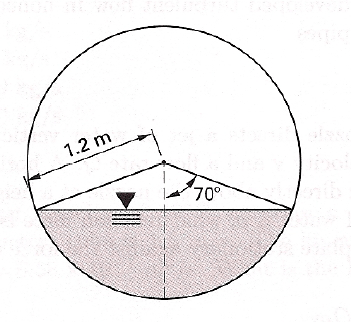
\includegraphics[width=3in]{CircularSewer.png}
   \caption{Circular channel flowing partially full.}
   \label{fig:CircularSewer} 
\end{figure}

What is the hydraulic radius of flow in the circular section?
%standard answer set
\begin{enumerate} [(A)]
\item $0.44$ m
\item $0.88$ m
\item $1.30$ m
\item $1.80$ m
\end{enumerate}
%====== SOLUTION ========
% A   geometry.  
% NCEES p 28
\clearpage
3. A storm sewer (reinforced concrete pipe) is 400-feet long and 30-inches in diameter.  The sewer flows full (but not-surcharged) between a personnel access shaft (invert elevation $101.00$ feet) and a lift station sump (invert elevation $100.00$ feet).  Assuming Manning's roughness coefficient is $0.013$ for all flow depths, the sewer capacity is about
%standard answer set
\begin{enumerate} [(A)]
\item  $4.2$ cfs
\item  $9.8$ cfs
\item  $20.5$ cfs
\item  $32.6$ cfs
\end{enumerate}
%====== SOLUTION ==========================
% C  use Manning's equation for full pipe flow
%  NCEES pp 160-161
%==========================================
%=======================================================================
\clearpage
4. A smooth concrete channel is depicted in Figure \ref{fig:TriangleChannel}.  The channel's dimensionless slope in the direction of flow is $0.005$.  If the flow width at the surface is $2$-meters, what is the flow rate in the channel using the Hazen-Williams friction formula?

\begin{figure}[h!] %  figure placement: here, top, bottom, or page
\centering
   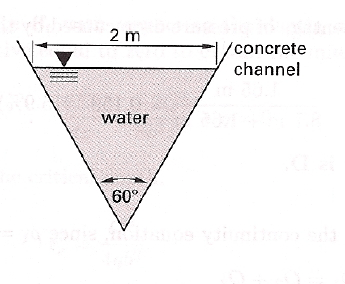
\includegraphics[width=3in]{TriangleChannel.png}
   \caption{Triangular channel.}
   \label{fig:TriangleChannel} 
\end{figure}

%standard answer set
\begin{enumerate} [(A)]
\item $0.8~\text{m}^3/\text{s}$
\item $1.3~\text{m}^3/\text{s}$
\item $6.8~\text{m}^3/\text{s}$
\item $9.8~\text{m}^3/\text{s}$
\end{enumerate}
~\clearpage
5. Water is pumped from a lake with a pipe inlet at elevation $200$-meters to a reservoir with elevation $205$-meters.  The pipeline from the lake to the reservoir is $300$-meters long, cast-iron, with $0.3$-meter inside diameter.  The flow rate in the pipe is $1.25~m^3/sec$.  The kinematic viscosity of water is $1 \times 10^{-6}~ m^2/sec$.  The roughness height for cast iron is $e=0.25~mm$.  Using the Darcy-Weisbach friction loss model, the pipe head loss is approximately
\begin{enumerate} [(A)]
\item 300 m
\item 310 m
\item 320 m
\item 330 m
\end{enumerate}
%====== SOLUTION =======
% B   Use moody chart, and roughness height.   enter chart using Re
% NCEES p 71,
% Also table of roughness
%========================
\clearpage
6.	The pressure drop over 15 m of 2-cm-diameter galvanized iron pipe (roughness height  = 0.25mm) is measured to be 60 kPa.  If the pipe is horizontal, estimate the flow rate of water.  ($\nu = 10^{-6} m^2/sec$)
\begin{enumerate} [(A)]
\item	6.82 L/s
\item 2.18 L/s
\item 0.682 L/s
\item	0.218 L/s
\end{enumerate}
~\clearpage
7.	What is the power requirement of an 85\% efficient pump that transports $0.04 m^3/sec$ of water if it increases the pressure from $200$ kPa to $1200$ kPa?
\begin{enumerate} [(A)]
\item	4.8 kW
\item	14.2 kW
\item	34.0 kW
\item	47.1 kW
\end{enumerate}
~\clearpage
8.) A water supply system draws from a river at an elevation of 800-feet and delivers the water to a storage reservoir at elevation 820-feet.  The supply pipeline is a 1000-foot long, 10-inch diameter, cast iron pipe.  Minor losses, entrance, and exit losses are neglected.  A single pump with the pump characteristic curve in Figure \ref{fig:PumpCurve} is used to fill the reservoir.

\begin{figure}[h!] %  figure placement: here, top, bottom, or page
\centering
   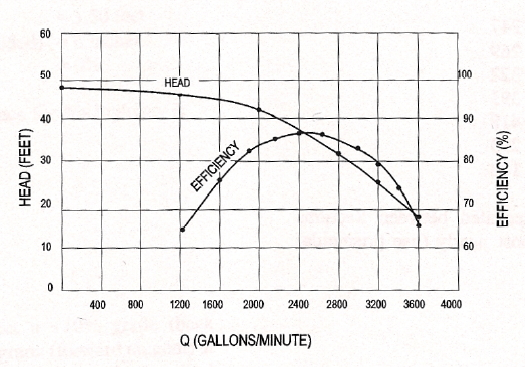
\includegraphics[width=4in]{PumpCurve.png}
   \caption{Pump characteristic curve}
   \label{fig:PumpCurve} 
\end{figure}

The system characteristics for the water supply are listed in Table \ref{tab:SystemCurve}. 
% Requires the booktabs if the memoir class is not being used
\begin{table}[htbp]
   \centering
      \caption{Pumped-Storage System Performance Characteristics.}

   \begin{tabular}{ccc} 
   ~&~&~\\
   Discharge (gpm) & System Loss (feet) & Pumping Head (feet) \\
   \hline
   \hline
   1,000 & 6.2 & 47 \\
   1,500 & 14.0 & 45 \\
      2,000 & 24.9 & 44 \\
         2,500 & 39.0 & 34 \\
            3,000 & 52.6 & 28 \\     
            \hline
   \end{tabular}
   \label{tab:SystemCurve}
\end{table}
\newpage

The operating point of the pump station is about
%standard answer set
\begin{enumerate}[(A)]
\item $1450$ gpm
\item $1875$ gpm
\item $2400$ gpm
\item $2800$ gpm
\end{enumerate}
~\clearpage
9. The electric power supplied to the pump to lift the water at the operating point is about\footnote{The efficiency on the pump curve is the wire-to-water efficiency}.
%standard answer set
\begin{enumerate}[(A)]
\item $10.0$ kilowatts
\item $15.0$ kilowatts
\item $20.0$ kilowatts
\item $25.0$ kilowatts
\end{enumerate}
~\newline
%====== SOLUTION ==========================
% C  Use P=Q*gamma*h/effic.
%  Read effic as 0.85 from curve.
%  Q = 2000 gpm * 0.002228 = cfs
%  gamma = 62.4
%  added head = 45 ft
%  convert ftlbs/sec to hp, then hp to watts.
% NCEES pp 66; 20; 
%==========================================
%===========================================================================
\end{document}  
~\newpage
\begin{figure}[h!] %  figure placement: here, top, bottom, or page
\centering
   \includegraphics[width=4in]{Manometer.jpg}
   \caption{Air-Mercury-Liquid manometer.  %Note: Circa 2009 these would be quite rare; Mercury has been replaced in industrial manometers with polymer blends and oils.  The concepts for analysis are unchanged.
   }
   \label{fig:Manometer} 
\end{figure}
4. A manometer is shown on Figure \ref{fig:Manometer} with $h_p=25$~cm and $h_m=63$~cm.  The pipe is filled with flowing oil with a specific gravity of $S.G. = 0.8$.  The specific gravity of Hg (mercury) is $S.G. = 13.6$.  Assume other conditions are at STP (standard temperature and pressure).

The gage pressure at point $A$ is about
%standard answer set
\begin{enumerate} [(A)]
\item  $-80$ kPa
\item $-86$ kPa
\item $-88$ kPa
\item  $-90$ kPa
\end{enumerate}
~\newline
%======= SOLUTION ===========
% B  Use liquid statics concepts and P=Gamma*h   Correct for different SG
% NCEES pp 68
%============================
%===========================================================================
~\newpage

~\newline



~\newpage

8. A reservoir with water surface elevation of $200$-meters drains through a $1$-meter diameter pipe at elevation $180$-meters.  The pipe outlet is a jet discharge to the atmosphere.  Total head loss in the pipe and fittings are $18$-meters.  Assuming the reservoir is large so that the water elevation is relatively constant, what is the approximate flow rate in the outlet pipe?
%standard answer set
\begin{enumerate} [(A)]
\item $5~m^3/sec$
\item $6~m^3/sec$
\item $30~m^3/sec$
\item $40~m^3/sec$
\end{enumerate}
~\newline
%====== SOLUTION ==========================
% A  Energy equation direct application.
% P in jet is set to 0 gage
% Solve for V, Q=VA
%  NCEES pp 65; 69
%==========================================

9. A fluid with a vapor pressure of $0.2$Pa and a specific gravity of $S.G.=12$ is used in a barometer.  If the fluid column height is $100$cm, what is the atmospheric pressure?
%standard answer set
\begin{figure}[h!] %  figure placement: here, top, bottom, or page
%   \includegraphics[width=2in]{fig4.pdf} 
\end{figure}
\begin{enumerate} [(A)]
\item $9.80$ kPa
\item $11.80$ kPa
\item $101$ kPa
\item $118$ kPa
\end{enumerate}
~\newline
%======= SOLUTION ============
% D   apply hydrostatic fluid with VP correction
% NCEES p 68
%============================

\newpage
10. A closed tank in Figure \ref{fig:TankPressure} contains water.  The air pressure above the water in the tank is $700$~kPa.  
\begin{figure}[h!] %  figure placement: here, top, bottom, or page
\centering
   \includegraphics[width=4in]{TankPressure.jpg}
   \caption{Closed, pressurized tank.}
   \label{fig:TankPressure} 
\end{figure}

What is the pressure at location $P$ in the tank, halfway up the inclined wall?
%standard answer set
\begin{figure}[h!] %  figure placement: here, top, bottom, or page
%   \includegraphics[width=2in]{fig5.pdf} 
\end{figure}
\begin{enumerate} [(A)]
\item $0.922$ MPa
\item $7.22$ MPa
\item $7.56$ MPa
\item $8.13$ MPa
\end{enumerate}
~\newline
%======= SOLUTION ============
% A   geometry and depth in a fluid.  Need to correct for atmospheric pressure.
% NCEES p 68
%============================
~\newpage

12. A nozzle directs a jet of water upward vertically with velocity $V$ and discharge $Q$.  A horizontal plate is located above the nozzle at distance $h$ from the nozzle.  If water density is $\rho$, what reaction force is required to keep the plate stationary against the force of water?
%standard answer set
\begin{enumerate} [(A)]
\item $Q\rho V$
\item $Q\rho \sqrt{2 g h}$
\item $\frac{Q \rho g h}{V}$
\item $Q \rho \sqrt{V^2 - 2 g h}$
\end{enumerate}
~\newline
%======= SOLUTION ======
% By inspection, D.  Only formula that accounts for mgy loss
% NCEES p
%===========================================
%=========================

~\newline
%====== SOLUTION =======
% NCEES p161 and geometry 
% A
%===================




16.	Bernoulli’s equation cannot be used to approximate the pressure drop for which of the following?	
%standard answer set
\begin{enumerate} [(A)]
\item across an orifice through which water flows
\item across a nozzle through which water flows
\item from the free stream to the stagnation point on an airfoil of a small aircraft
\item across a Venturi meter
\end{enumerate}
~\newline


~\newline


~\newline
\textbf{STOP!}  

This is the end of \textbf{Hydraulics and Hydrologic Systems Training Quiz}.

If you complete this quiz in less than 40 minutes, you may return to any of the problems.


~\newline
%===== SOLUTION ========================
%    C   use pipe-loss formulas and energy equation.
%    NCEES pp 65-66
%=======================================
9.	The pressure drop across a valve, through which $0.04~m^3/sec$ of water flows, is measured to be $100$ kPa.  Estimate the loss coefficient if the nominal diameter of the valve is $8$ cm.
\begin{enumerate} [(A)]
\item	0.32
\item	0.79
\item	3.2
\item	8.7
\end{enumerate}
~\newline